\documentclass[10pt]{beamer}

\usetheme[progressbar=frametitle]{metropolis}
\usepackage{appendixnumberbeamer}

\usepackage{booktabs}
\usepackage[scale=2]{ccicons}

\usepackage{pgfplots}
\usepgfplotslibrary{dateplot}

\usepackage{xspace}
\newcommand{\themename}{\textbf{\textsc{metropolis}}\xspace}

\title{67301 - MULTI ROBOT SYSTEMS - Spring 2021}
\subtitle{Final project presentation}
\date{}
\author{Tamer Ghattas}
\institute{
The Hebrew University of Jerusalem School of Computer Science and Engineering
}
% \titlegraphic{\hfill\includegraphics[height=1.5cm]{logo.pdf}}

\begin{document}

\maketitle


\section{Single-agent dirt collection}

\begin{frame}{Single-agent dirt collection}
\begin{itemize}
    \item {\bf Problem description:} collect as many as possible dirt pieces from an unknown environment without having the option of sensing the dirt. 
    \item That can be translated to: we need to cover diverse areas in the room in the shortest period of time.
    \item The problem is hard because with the time limitation we often inherit an upper bound for the area coverage.
    \item An exhaustive approach to the solution would be moving sequentially along every accessible point known from the map in hand competing a perfect coverage.
\end{itemize}
\end{frame}


\begin{frame}{Single-agent dirt collection}

We model the problem as a graph $G=(V, E)$ where the nodes $V$ represent a pixel in the map and $E$ and edge existing between every adjacent pair of pixels (nodes).


\bigskip


Our suggested solution takes the graph as input and derive goals for the robot aiming for diverse area coverage.
\end{frame}


\begin{frame}{Single-agent dirt collection}

We implemented our approach using image processing manipulations on the binary image of the given map:
\graphicspath{{images/}}
\begin{itemize}
    \item First we generate black & white image from the map structure.
    \item Then we perform Euclidean Distance Transform on the image.
    \item Now, we have range of gray levels that are distributed among pixels as a function their distance of the nearest black pixel, i.e the nearest wall.
    \bigskip
    
    \begin{figure}[htp]
    \centering
    \includegraphics[height=3cm,width=4cm]{map}
    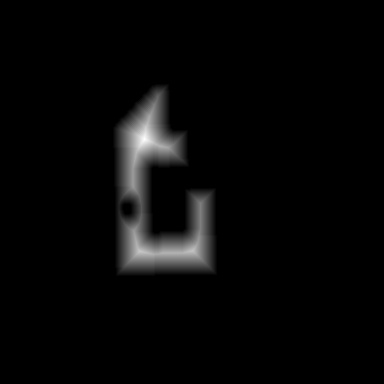
\includegraphics[height=3cm,width=4cm]{edt_img}

    \label{fig:galaxy}
\end{figure}
    
\end{itemize}

% \bigskip 

% We evaluated our approach by  TODO!!!

\end{frame}

\begin{frame}{Single-agent dirt collection}

\begin{itemize}
    \item This approach was the second, first I thought about using Zig-Zag pattern with a randomly sampled angle on each turn but that is prone to missing parts of certain room structures.
    \item The presented approach on average, covers all parts of the room after enough time.
    \item A good approach might be to partition the map into compact clusters and run zig-zag like pattern on each.
\end{itemize}

\end{frame}


\section{Single-agent inspection}

\section{Multi-agent dirt collection}

\section{Multi-agent dirt inspection}

\section{Conclusion}



\end{document}
